\label{cha:design_of_data_and_functionality}

\subsection{Excercise CarRentalEntities}
\label{sec:exercise_car_rental_entities}
\subsubsection*{Description of the Initial Entity Diagram}
The entity diagram consists of the following entities:
\begin{itemize}
    \item Customer entity
    \item Rental entity
    \item Car entity
    \item Date value object
\end{itemize}
A customer has zero ore more rentals.
Each rental has a date value object and belongs to at most one car.

\subsubsection*{Adding the Attributes}
The extended entity diagram is shown in figure \ref{fig:extendedEntityDiagram}.
The following attributes are added to the entities:
\begin{itemize}
    \item Customer entity
    \begin{itemize}
        \item id: contains the customer id and identifies the customer
        \item name: contains the name of the customer
        \item creditCard: true if the customer has a valid credit card, false otherwise
        \item rentals: list of rental objects that belong to the customer. The list can be empty if no cars are rented.
    \end{itemize}
    \item Rental entity
    \begin{itemize}
        \item id: contains the rental id and identifies the rental
        \item date: link to the date value object that contains the start and end date of the rental
        \item car: link to the car object that is rented. Can be null if no car is assigned to the rental
    \end{itemize}
    \item Car entity
    \begin{itemize}
        \item id: contains the car id and identifies the car
        \item type: contains the type of the car
        \item rented: true if the car is rented, false otherwise
        \item price: contains the price of the car per day
    \end{itemize}
    \item Date value object
    \begin{itemize}
        \item startDate: contains the start date of the rental
        \item endDate: contains the end date of the rental
    \end{itemize}
\end{itemize}

\begin{figure}[h]
    \centering
    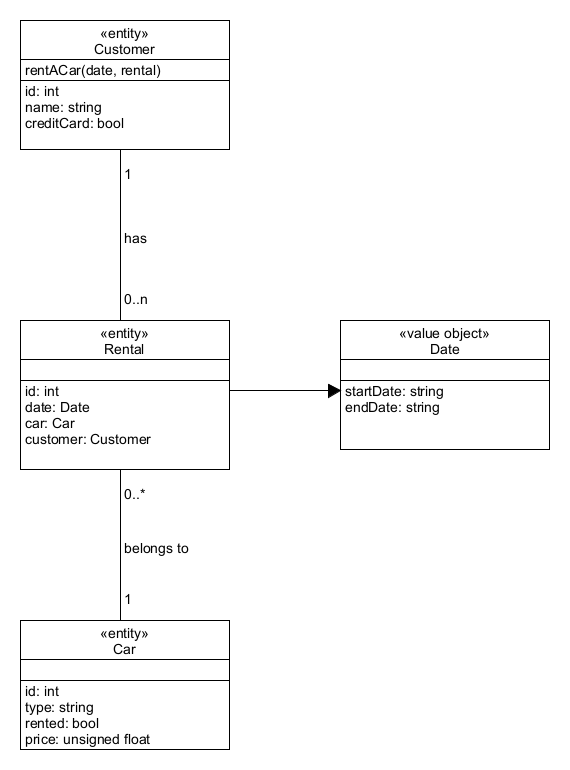
\includegraphics[width=0.6\textwidth]{figures/goLang/carRental/carRental_extendedEntity.png}
    \caption{Extended Entity Diagram}
    \label{fig:extendedEntityDiagram}
\end{figure}

\subsubsection*{Adding the Functionality as a Method}
The chosen signature of the funcion is \texttt{rentACar(date, rental)}.
The method works as follows:
\begin{enumerate}
    \item The function checks, if the credit card is valid. If not, the function aborts.
    \item The date object is created with the given start and end date and is given to the function.
    \item The given rental object is assigned according to the chosen car / rental.
    \item The algorithm checks, if the car assigned to the rental is available. If not, the function aborts.
    \item The car is marked as rented.
    \item The date object is assigned to the rental.
    \item The rental object is linked to the customer.
    \item All changes are saved to the objects.
\end{enumerate}

\subsection{Excercise CarRentalExampleData}
\label{sec:exercise_car_rental_example_data}
\subsubsection*{Analyze Alice's Rental Request}
Yes, the request is successful for the following reasons:
\begin{itemize}
    \item The car exists
    \item The car is not rented for the specified time period
    \item Alice is not registered yet, but will be added to the customers table
\end{itemize}
Therefore the request is successful and the car is rented to Alice.

\subsubsection*{Write YAML Code}
-- Still needs to be done --